\section{OpenNMS Community}
In \emph{OpenNMS} we have a global community consisting of developers, corporations, service providers, researchers and users.

\subsection{OpenNMS Developers}

\subsubsection{JIRA ID}
\emph{Atlassian JIRA} is the "home" for the project management and its developers: create a \emph{JIRA ID} on \url{http://issues.opennms.org/secure/Signup!default.jspa} if you don’t have one already. You’ll need it to report bugs, issues or enhancements.

\subsubsection{Licensing}
If you are a developer interested in contributing to the OpenNMS project you will need to sign the \emph{OpenNMS Contributor Agreement (OCA)}. If you are contributing on behalf of a company, an authorized representative of your company should also sign the \emph{OCA}. You find the instructions and the agreement on \url{http://www.opennms.org/wiki/Contributor_Agreement}.

%\subsubsection{Contributor's wiki}

\subsubsection{Core Principles}
Familiarize yourself with \emph{OpenNMS} principles:
\begin{enumerate}
  \item \textbf{\textcolor{red}{What "Open" means \url{http://wiki.openstack.org/Open}}}
  \item \textbf{\textcolor{red}{Design tenets \url{http://wiki.openstack.org/BasicDesignTenets}}}
  \item \textbf{\textcolor{red}{Coding standards \url{http://wiki.openstack.org/CodingStandards}}}
  \item \textbf{\textcolor{red}{The release cycle \url{http://wiki.openstack.org/ReleaseCycle}}}
  \item \textbf{\textcolor{red}{The OpenStack branch model \url{http://wiki.openstack.org/BranchModel}}}
\end{enumerate}

\subsubsection{Get the Code}
The source code is hosted on \emph{GitHub} on \url{https://github.com/opennms}. Code contributions can be merged into \emph{OpenNMS} with \emph{pull requests}. The workflow to get your source code into \emph{OpenNMS} is shown in picture \ref{fig:contrib-workflow} on page \pageref{fig:contrib-workflow}.

\begin{figure}[h]
	\centering
	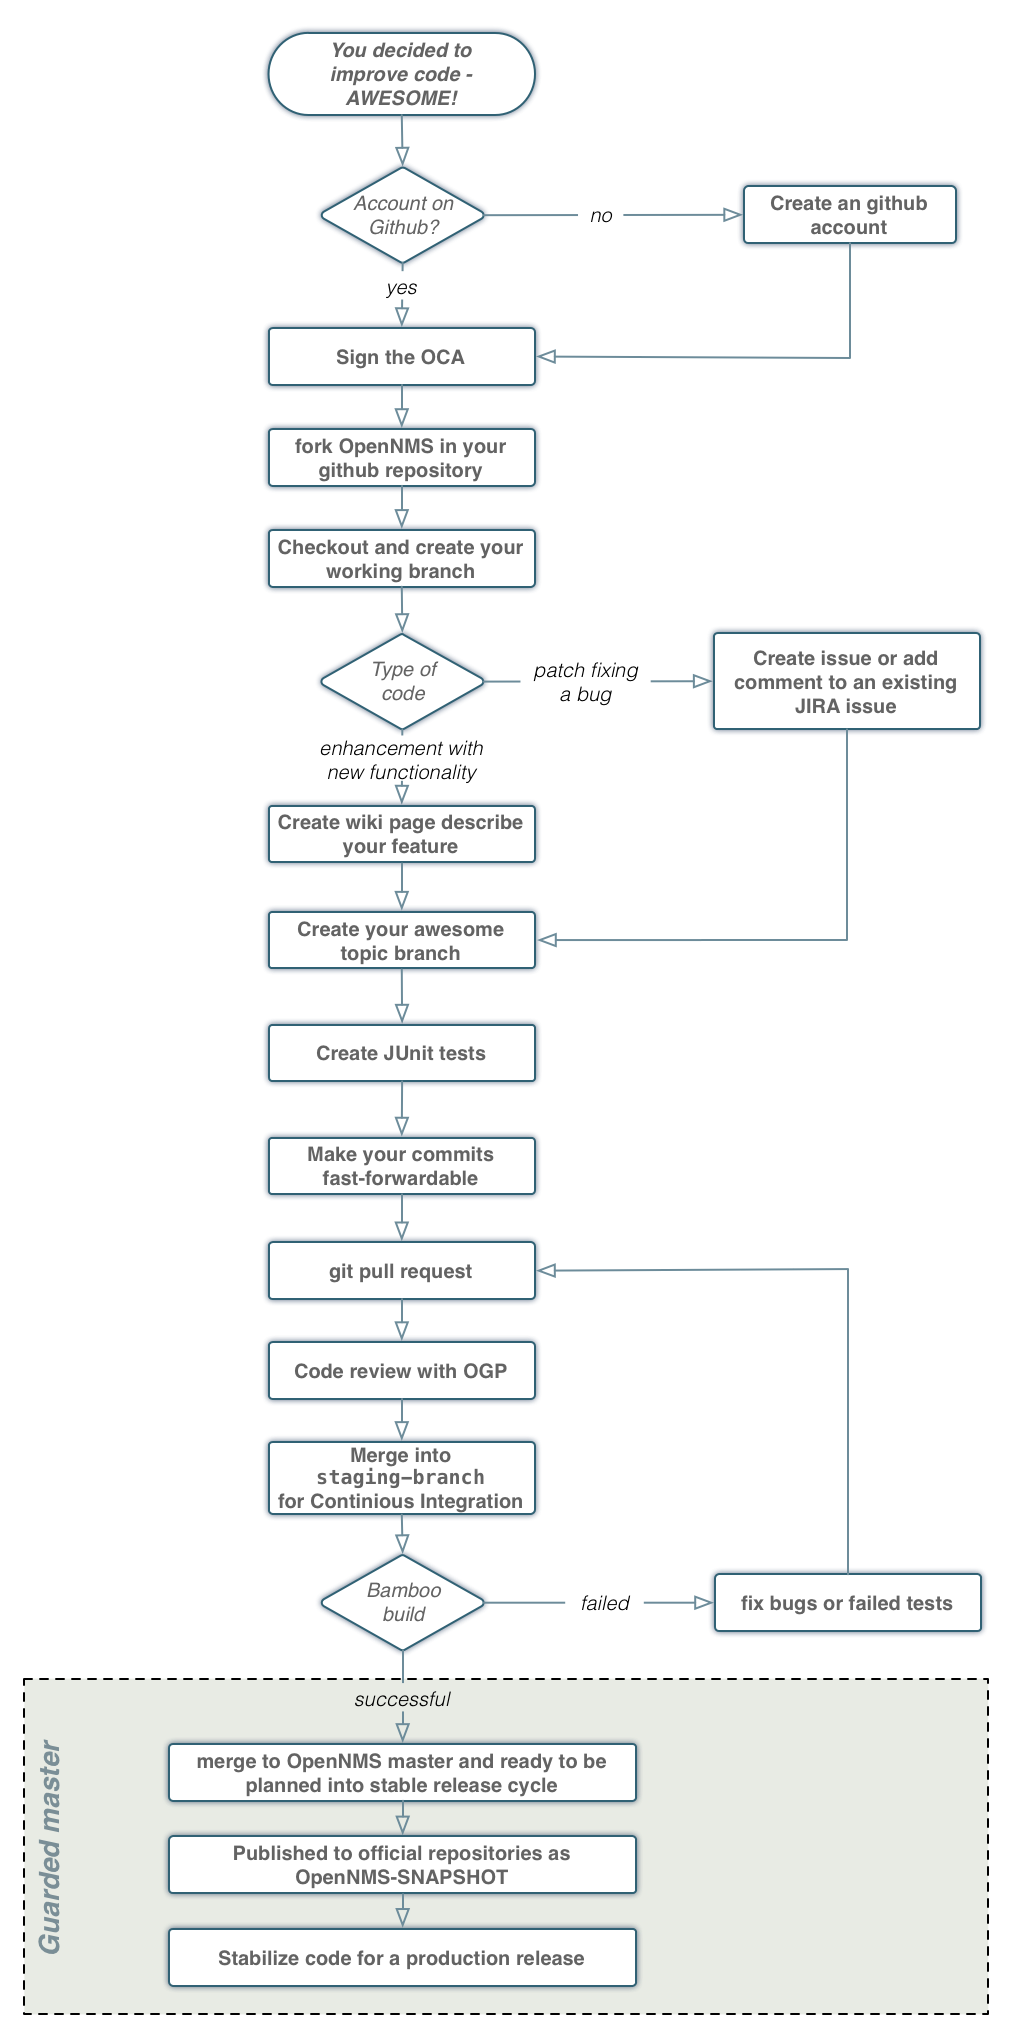
\includegraphics[width=0.75\textwidth]{images/contribution-workflow.png}
	\caption{Workflow for code contribution}
	\label{fig:contrib-workflow}
\end{figure}

\subsubsection{Bugs}
Bugs can be a good place to get your coding feet wet. \textbf{\textcolor{red}{The bugs confirmed and triaged that should be simple to tackle are tagged 'low hanging fruit' \url{https://bugs.launchpad.net/openstack/+bugs?field.tag=low-hanging-fruit} - THIS IS NICE}}

\subsubsection{Other good resources for developers}
\begin{itemize}
  \item Development Mailing List: \url{https://lists.sourceforge.net/lists/listinfo/opennms-devel}
  \item IRC \#opennms on Freenode \url{http://webchat.freenode.net/}
  \item \textbf{\textcolor{red}{Project meetings held publicly on IRC, Google Hangouts, other ideas?!}}
\end{itemize}

\subsection{Documentation}
\begin{itemize}
  \item Getting Started Get up and running quickly with \emph{OpenNMS} you can use \emph{VirtualBox}\footnote{VirtualBox web site: \url{https://www.virtualbox.org/}} and \emph{Vagrant}\footnote{Vagrant web site: \url{http://www.vagrantup.com/}} which is documented on \url{http://www.opennms.org/wiki/OpenNMS_and_Vagrant_with_VirtualBox}.
  \item Install on \emph{OpenNMS} on \emph{Debian/Ubuntu} is documented on \url{http://www.opennms.org/wiki/Installation:Debian}
  \item Install on \emph{OpenNMS} based systems on \emph{CentOS/RedHat} is documented on \url{http://www.opennms.org/wiki/Installation:Yum}
  \item General installation documentation can be found on \url{http://www.opennms.org/documentation/installguide.html}
  \item \textbf{\textcolor{red}{LINK to operational documentation}}
  \item \textbf{\textcolor{red}{LINK to developer documentation}}
  \item \textbf{\textcolor{red}{LINK to API documentation on the \emph{RESTful APIs} provided by \emph{OpenNMS}}}
  \item \textbf{\textcolor{red}{Link to glossary with a list of terms and their definition}}
\end{itemize}

\subsubsection{Contribute to Documentation}
\textbf{\textcolor{red}{At the core of OpenStack is the community and collaboration that we do - the same rules for the code apply to documentation too. Ideally any code contribution that is merged into the base has documentation to go with it. Anne Gentle is the coordinator for all documentation efforts, both community-based and "official" docs. The page \url{http://wiki.openstack.org/Documentation/HowTo} describes the methods we use to create the basis for world-class documentation for OpenStack developers and users. A GUESS WE DONT HAVE SOMETHING}}

\subsection{OpenNMS Ecosystem}
A robust ecosystem is essential to \emph{OpenNMS’s} success. There are several ways your company can join this growing and vibrant ecosystem.

\subsubsection{Sponsor the OpenNMS Foundation}
Organizations can apply to become new members. You can join as an individual or as a company member. Details on membership can be found on \url{http://www.opennms.eu/membership}.

\subsubsection{Individual Member of the Foundation}
Any person can join the \emph{OFE}. As an individual member you can get active in the \emph{OpenNMS} community as a user, developer, business person, art maker, or however else you want to contribute.

% \subsubsection{OpenNMS User Groups}
% We don't have one yet

\subsection{Other userful tools}

\subsubsection{Questions and Answers (ask.opennms.eu)}
The place where people can ask questions and give answers about \emph{OpenNMS} deployments, operations and development is \url{http://ask.opennms.eu}.

\subsubsection{Wiki}
A lot of good information on getting started with the \emph{OpenNMS} project can be found in the wiki. The search function in the upper right hand corner of the wiki is very powerful and searches both by title and content. The wiki entry can be found at \url{http://www.opennms.org/wiki/Main_Page}. In the left navigation menu you can also find links to official documentation, white papers and FAQs.

\subsubsection{Bug Reporting}
The \emph{OpenNMS} community appreciates testers and their feedback. To report a bug you must first sign up for a \emph{JIRA} account. Check that the bug you found has not already been reported by searching \emph{JIRAs} bugs list: \url{http://issues.opennms.org}. In the top menu \emph{Issues}, you can use \emph{Search for Issues} in the project \emph{OpenNMS} with \emph{Type: Bug}.

If you found a new bug, fill out a bug report:
\begin{itemize}
  \item Give a clear, concise summary.
  \item Provide as much detail as possible in the description. Paste in your command output or stack traces, link to screenshots, etc.
  \item Be sure to include which version of the software you are using. This is especially critical if you are using a development or unstable branch.
  \item Add information about your Java environment which is used by OpenNMS. You can find it in the configuration \texttt{java.conf} in your OpenNMS configuration directory and by running \texttt{java -version} 
  \item Any deployment-specific info is helpful as well. Example: Ubuntu 10.04, which version of PostgreSQL, JRobin, RRDtool, store-by-group- or store-by-foreignsource settings.
\end{itemize}

\subsubsection{Keeping in touch}
\begin{itemize}
  \item Twitter: @opennms
  \item Blogs of users and developers: \url{http://planet.opennms.org/}
  \item Developers hold real-time discussions at Internet Relay Chat (IRC). Channel \#openstack on Freenode (\url{http://webchat.freenode.net} via browser client)
  \item YouTube Channel with videos from conferences: \url{http://www.youtube.com/user/opennms}
  \item Last conference material and slides from OUCE 2013: \url{http://ouce.opennms.eu/en/ouce2013/public/events}
\end{itemize}

\subsubsection{Mailing Lists}
The project runs many mailing lists. All our important mailing lists can be found on the wiki page \url{http://www.opennms.org/wiki/Mailing_lists}. The most used traffic is on the lists \emph{opennms-discuss}, \emph{opennms-install} and \emph{opennms-devel}. The list \emph{opennms-announce} is meant to be a low traffic list.

\subsection*{The OpenNMS Group, Inc.}
The OpenNMS Group, Inc. is the biggest sponsor of the project. The software itself is licensed under GPLv3+. The company \emph{The OpenNMS Group, Inc.} provides professional support and gives those people a place who want to spend significant time of their life to the project. Code development in commercial environment is reflected as a code contribution to the free software project. Besides code contribution, there are other topics like packaging and continuos integration which is also provided publicly to the project.

\subsection*{Order of the Green Polo}
The Order of the Green Polo (OGP) is the super secret brotherhood of developers of the \emph{OpenNMS Project}. You can recognize and \emph{OGP} member by their good looks as well as their super-flashy, very coveted \emph{OpenNMS Green Polo}. As Tarus Balog said:
 
\begin{quote}
Back in fall of 2004, I wanted to find a way to recognize those people who make \emph{OpenNMS} what it is, and to thank them in some fashion. 
Ever since the advent of "business casual" workplace attire, the "logo" polo shirt has become a fixture in IT departments around the world. We sell black and white polos with the \emph{OpenNMS} logo on our web site.

But this is much, much, much, different. These are "green" polos, very rare, and they will never be available for sale. Think of them as equivalent to winning \emph{The Masters} golf tournament's green jacket - only harder to get.
In order to get one, all one has to do is give up all hope of having a life outside of \emph{OpenNMS}, work long hours for free, and basically become a closed superhero, squashing bugs (or uncovering existence) in a single bound.
\end{quote}

\subsection*{OpenNMS Foundation Europe}
The \emph{OpenNMS Foundation Europe e.V.} (OFE) was founded on July 31st, 2012. OFE is a registered non-profit organization in Germany. The objective of the organization is to promote, develop, educate and research around free software and network (management) technologies, especially \emph{OpenNMS}. To do this, the \emph{OFE} organizes the OpenNMS User Conference Europe (OUCE) run by foundation members and volunteers. The OFE web site with links to material of the conference can be found at \url{http://www.opennms.eu}.
